\chapter{Implementation}

In this chapter the technologies used during the project are explained. An overview of how the design laid down in chapter 3 was implemented is presented.
Any challenges that were faced during the implementation are also discussed and contrasted with alternative approaches.

\section{Technologies}
Following an investigation of the field and the available technologies it was decided that the system would be implemented in Python.
Python is a dynamically typed language which has support for multiple different programming paradigms.
Python is widely used today both in industry and the scientific community.
Libraries such as NumPy, SciPy, matplotlib and pandas are widely used in the fields of data-analysis and scientific computing.
This has proven that Python is an adequate substitute for languages such as C, C++, Java, R, Matlab, etc\cite{PythonR}.

Python also favors readability and minimalism compared to low level programming languages.
Despite being a relatively high level programming language, Python can also interface with C and C++ using the Cython library.
This is particularly useful when making code optimisations, such as vectorising code loops.

\subsection{Gensim}
Gensim is a Python toolkit for topic modeling and semantic analysis of textual data.
Gensim favours an online approach to training the models.
This is achieved using Python generator expressions, which can result in only one document from the corpus residing in main memory at any one time.
This small memory footprint and incremental approach allows Gensim to scale in relation to the size of the corpus.
Gensim interfaces very well with NumPy and SciPy libraries.
As well as this, it has been optimised to use the Cython library in order to speed up execution.

By using the Gensim toolkit the system was able to gain access to the following tools:
\begin{itemize}
    \item build a dictionary of features from the corpus
    \item convert the corpus to a bow representation
    \item apply tf-idf transformations to bow models
    \item train LDA on bow models
    \item convert bow models to NumPy arrays
    \item train Miklov's Word2Vec model
    \item easily load and save different representations of the corpus
    \item use Gensim's native indexing for document similarities
\end{itemize}

As shown above Gensim is quite extensive in it's functionality and thus allowed the easy manipulation of corpus.
Without access to Gensim it would have taken a considerable amount of time to implement all of this functionality.

\subsection{Annoy}
Annoy is a C++ library with Python bindings for approximate-Nearest-Neighbour search.
Annoy was created by Spotify to generate recommendations.
Within Spotify they use it to find similar users and similar songs.
Spotify's system contains millions of tracks and has approximately 60 million active users.
This shows that Annoy is a tried and tested approximate-Nearest-Neighbour library which has scaled to large data-sets.

Annoy does approximate-Nearest-Neighbour queries by building an index using locality sensitive hashing (LSH) and random projections.
LSH is a technique used to reduce the dimensionality of high dimensional data by mapping the data into hash bins.
LSH tries to map similar items into the same bin and is very different to cryptographic functions which try to reduce the possibilities of collisions\cite{slaney2008locality}.
Random projections are a type of dimensionality reduction techniques which work by projecting the data into a random subspace of lower dimension\cite{Dasgupta2000}.

Radim {\v R}eh{\r u}{\v r}ek, the creator of Gensim investigated the performance of different nearest neighbor libraries in November 2013 \cite{radimKnnInvestigation}.
In the final investigation the libraries were reduced down to just Annoy and FLANN.
During that investigation, Radim found that the query time for FLANN was approximately four times quicker than Annoy.
Annoy on the other hand had almost perfect accuracy (When compared to a non-approximate version of k-NN) compared to FLANN.

Annoy was selected for the k-NN investigation as it:
\begin{itemize}
    \item Was found to be the most accurate approximate-Nearest-Neighbour library
    \item has an easy to understand API
    \item Will be integrated into Gensim once the Boost library has been dropped as a requirement
    \item Has been shown to scale to very large data-sets
\end{itemize}

As shown above Annoy was chosen largely due to it's simplicity and the ease of integration with the Gensim toolkit.

\section{System Implementation}
In this section an outline the system that was built, as prescribed in Chapter 3, is presented.
Where possible UML has been used to describe the relations between the different components of the system.

\subsection{System}
\begin{figure}[h]
    \centering
        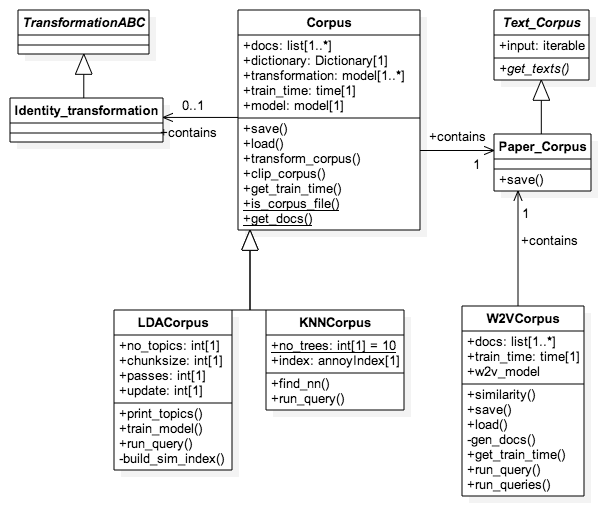
\includegraphics[width=0.7\textwidth]{Figures/FYPClassDiagram.png}
    \caption{System class diagram}
    \label{fig:UMLClass}
\end{figure}

Figure~\ref{fig:UMLClass} presents an overview of the system as a UML class diagram.
The main class in the system is the Corpus class.
The Corpus class is an abstract class used to represent a bag-of-words corpus.
The docs attribute is a list of document names from the corpus.
The dictionary attribute is a Gensim Dictionary object which represents the words in the corpus and their respective term frequencies.

The Corpus classes static function get\_docs is an interesting function used to generate a list of corpus files.
The function receives a path to a system directory, a dictionary of file distributions in sub-directories and a maximum number of files.
This function then generates a list of files from each of the sub-directory while maintaining the specified distributions.
The function then returns this flattened list of file paths.
This function is useful as it ensures that the same proportion of files will be sampled from each arXiv defined topic area, no matter the size of the corpus currently being tested.

The transformation attribute is used to represent transformation that have been applied to the bag-of-words corpus.
An interesting feature of Gensim is that you can stack corpus transformations on top of each other.
This for example could be used to apply a tf-idf transformation followed by an Latent-Semantic-Indexing transformation.
This however poised a small problem for the system.

When creating the above system, code readability and code reuse were huge factors that were considered.
In an earlier version of the project, if the corpus had a transformation applied, the transformation was only executed when iterating through the corpus.
However if a corpus did not have any transformations applied to it, this required an nested if-statement, which reduced code readability.

An alternative to this was to create an identity transformation which inherited from Gensim's TransformationABC class.
This Identity\_transformation is basically an identity function which returns the input document vector.
This approach was based on monad transformers from Haskell where the inner-most monad of stacked monad-transformers is either the identity monad or an IO action.
This eliminated the unnecessary conditional statement and increased the code readability by applying functional programming paradigms.

The Paper\_Corpus class is a wrapper around Gensim's Text\_Corpus class.
Gensim favours document streaming and is agnostic as to how the corpus is stored.
The corpus could be stored in one file or distributed across the web.
The Text\_Corpus is an abstract class which allows the user to use Python's generator expressions to lazily load documents from the corpus and do any necessary pre-processing to the text.
As the arXiv corpus being investigated is organised as a collection of .txt files in multiple directories, this approach allowed the system to load documents one at a time and do some pre-processing to the text.
The pre-processing conducted includes; reading the document into memory, translating the text to lower-case, splitting the word-tokens on whitespace characters, and filtering out words that appear only once in the document.

Both the LDACorpus and the KNNCorpus files use a bag-of-words representation of the corpus and thus inherit from the Corpus class.
W2VCorpus on the other hand trains it's model using the plaintext corpus.
As stated above when implementing the system, code reuse and readability were two of the main factors considered.
When it came to implementing the Word2Vec model a choice was made to not inherit from the Corpus class even though there was some shared functionality.
This decision was made largely due to the difference in the semantics of the Word2Vec model and the models which used a bag-of-words representation.
This of course means that the DRY principle, from software-engineering, is violated but the shared functionality between the two classes is minor and separation ultimately increases the overall readability of the code.

The LDACorpus and the KNNCorpus are relatively small classes which inherit the majority of their functionality from the Corpus class.
The attributes for the LDA class and the k-NN expose the API for the underlying models imported from the Gensim and Annoy libraries.
Exposing the API allowed easier testing and tweaking of the algorithms being investigated.

\subsection{Code Harnesses}
Two code harnesses are used in the research project. The first harness is used to generate the LDA, k-NN and Word2Vec corpora and to log the time taken to generate each corpus.
The second harness is used to run similarity queries on each of the corpus files, log the time taken to run the similarity queries, log the results of each of the queries and then output the results in JSON.

\subsubsection{Generation Harness}
The generation harness is useful for the creation of corpora of varying size.
From the command line the script receives a list of corpus sizes to create, a corpus source directory and the algorithm to apply to the corpus.
An optional directory can also be passed as an argument to the script.
This optional directory is an output directory to store the generate corpus and model files.
If this directory is not specified a directory is created where the script is run and all files generated are stored in it instead.

The generation harness iterates through the list of corpus sizes and creates a corpus of that size.
For all of the algorithm apart from Word2Vec, a dictionary must be created and the corpus must be converted to a bag-of-words representation.
Word2Vec effectively skips this stage as it builds it's dictionary and model in the training stage.
For each corpus created, the time take to build the corpus is logged to a log file.
After the corpus and dictionary files have been created, the models is trained.
As Word2Vec differs from LDA and k-NN it trains using the original textual corpus.
LDA and k-NN on the other hand must use the dictionaries and bag-of-words representations created previously to train their models.
The times take to train each of the models is also logged to a file.

\subsubsection{Similarity Harness}
The similarity harness automates the process of using the models, which were generated by the generation harness, to query for similar documents.
The command line arguments for the similarity harness are very similar to the generation harness.
The script receives a list of corpus sizes, a directory of query files, a directory containing the previously generated models and the algorithm being tested.

For each of the sizes passed to the script, the list of query files is processed into the appropriate data representation.
For LDA and k-NN, the dictionaries created previously are loaded and the files from the query directory are converted to a bag-of-words representation.
For Word2Vec the process is slightly different because we need to find the word vector representations of the query documents before we can find similar documents.
This is achieved by loading the query documents and then adding them to the Word2Vec model.
This allows us to get a vector representation of the document which can be used to find similar words and similar documents.

The similarity queries are then run on each of the documents from the query corpus.
The time take to run the queries are logged to a file for later analysis.
The similar document results are also stored and later parsed to into readable JSON.
The similarity results are parsed into JSON in order to make them more portable.
This was done as there are some interesting Javascript libraries which could be used to visualise the results.

\section{Conclusion}
In this chapter the implementation of the system designed in chapter three has been described.
Any challenges encountered have been stated and their solutions explained.
A complete system for building models of a corpus and for querying the generated models has been built.
This consists of components to:
\begin{itemize}
    \item process a large number PDF documents into plain text
    \item to sample a distribution of documents from the corpus
    \item convert documents into a bag-of-words representation
    \item build models of the corpus
    \item time the execution for building and querying the models
    \item query the generated models using a collection of plain text documents
    \item parse and log similarity results
    \item and to visualise the data generated
\end{itemize}
This systems allows the easy analysis of machine learning algorithms on a textual corpus.
The system was originally intended for the arXiv corpus and the three machine learning algorithms stated previously. However, the system could be easily extended to use another text corpus or different algorithms.

In the following chapter, the results generated from the above system will be presented and analysed.
